\documentclass[article]{article}

% --- PACKAGES ---
\usepackage[margin=1in]{geometry}
\usepackage{amsmath}
\usepackage{amssymb}
\usepackage{graphicx}
\usepackage{booktabs} % For professional tables
\usepackage{siunitx}  % For formatting units
\usepackage{tikz}
\usepackage{pgfplots}
\usepackage{hyperref}

% --- PGFPLOTS SETUP ---
\pgfplotsset{compat=1.17}
\usetikzlibrary{arrows.meta}

% --- DOCUMENT ---
\title{Concise Notes: Thermodynamic Processes and Entropy}
\author{Gemini AI}
\date{\today}

\begin{document}

\maketitle

\section{The Foundation: The First Law of Thermodynamics}

This is the starting point for all energy changes. It's simply the \textbf{conservation of energy}.

\begin{itemize}
    \item \textbf{Concept:} The change in a system's \textbf{internal energy ($\Delta U$)} is equal to the \textbf{heat added to the system ($Q$)} minus the \textbf{work done by the system ($W$)}.
    \item \textbf{Core Equation:}
        $$ \Delta U = Q - W $$
    \item \textbf{Sign Convention (Crucial!):}
    \begin{itemize}
        \item \textbf{$\Delta U$ (Internal Energy):} The total energy stored in the gas molecules. For an ideal gas, it \textbf{only depends on temperature}.
            \begin{itemize}
                \item $\Delta U > 0$: Temperature increases.
                \item $\Delta U < 0$: Temperature decreases.
                \item $\Delta U = 0$: Temperature is constant.
            \end{itemize}
        \item \textbf{$Q$ (Heat):} Energy transferred due to a temperature difference.
            \begin{itemize}
                \item $Q > 0$: Heat flows \textbf{into} the system.
                \item $Q < 0$: Heat flows \textbf{out of} the system.
            \end{itemize}
        \item \textbf{$W$ (Work):} Energy transferred by expansion or compression.
            \begin{itemize}
                \item $W > 0$: System does work (expands, $V_{\text{final}} > V_{\text{initial}}$).
                \item $W < 0$: Work is done on the system (compresses, $V_{\text{final}} < V_{\text{initial}}$).
            \end{itemize}
    \end{itemize}
    \item \textbf{Key Gas Equations:}
    \begin{itemize}
        \item \textbf{Internal Energy Change:} $\Delta U = nC_v\Delta T$
            \begin{itemize}
                \item $n$ = moles of gas
                \item $C_v$ = specific heat at constant volume
                \item $\Delta T$ = change in temperature ($T_{\text{final}} - T_{\text{initial}}$)
            \end{itemize}
        \item \textbf{Work (general):} $W = \int P \, dV$ (Work is the area under the P-V curve).
    \end{itemize}
\end{itemize}

\hrule

\section{Specific Heats ($C_v$ \& $C_p$) \& Gas Structure}

This is how we \textit{quantify} the internal energy change and connect it to the gas's structure.

\begin{itemize}
    \item \textbf{Concept:} "Specific Heat" is the energy needed to raise the temperature of a gas. We use two types:
    \begin{itemize}
        \item \textbf{$C_v$ (Molar heat capacity at constant volume):} Used to find the change in internal energy. This is the \textit{only} one you need for $\Delta U$.
            $$\Delta U = nC_v\Delta T$$
        \item \textbf{$C_p$ (Molar heat capacity at constant pressure):} Used to find the heat added \textit{at constant pressure} ($Q_p$).
            $$Q_p = nC_p\Delta T$$
    \end{itemize}
    \item \textbf{Why is $C_p > C_v$?}
    \begin{itemize}
        \item At \textbf{constant volume} (using $C_v$), all the heat you add ($Q$) goes directly into raising the internal energy ($\Delta U$). No work is done ($W=0$).
        \item At \textbf{constant pressure} (using $C_p$), when you add heat, the gas \textit{also} expands and does work ($W > 0$). So, you must add \textit{more} heat to get the same temperature change, because some energy "leaves" as work.
    \end{itemize}
    \item \textbf{Key Relation (Mayer's Relation):} $C_p = C_v + R$ (where $R$ is the ideal gas constant, $\SI{8.314}{J/mol\cdot K}$)
    \item \textbf{Values (from Equipartition Theorem):} $C_v$ depends on the "degrees of freedom" ($f$)—how a molecule can move (translate, rotate). $C_v = (f/2)R$.
    \begin{itemize}
        \item \textbf{Monatomic Gas} (e.g., He, Ne, Ar)
            \begin{itemize}
                \item $f = 3$ (3 translations: x, y, z)
                \item $C_v = \frac{3}{2}R$
                \item $C_p = C_v + R = \frac{5}{2}R$
            \end{itemize}
        \item \textbf{Diatomic Gas} (e.g., N$_2$, O$_2$, H$_2$)
            \begin{itemize}
                \item $f = 5$ (3 translations + 2 rotations)
                \item $C_v = \frac{5}{2}R$
                \item $C_p = C_v + R = \frac{7}{2}R$
            \end{itemize}
        \item \textbf{Polyatomic Gas (non-linear)} (e.g., H$_2$O, CH$_4$)
            \begin{itemize}
                \item $f = 6$ (3 translations + 3 rotations)
                \item $C_v = 3R$
                \item $C_p = C_v + R = 4R$
            \end{itemize}
    \end{itemize}
\end{itemize}

\hrule

\section{Process 1: Isothermal ("Constant Temperature")}

\begin{itemize}
    \item \textbf{Definition:} A process that occurs at a constant temperature.
    \begin{itemize}
        \item $\Delta T = 0$
        \item Imagine the system is in a water bath that keeps its temperature fixed.
    \end{itemize}
\end{itemize}

\begin{figure}[h]
\centering
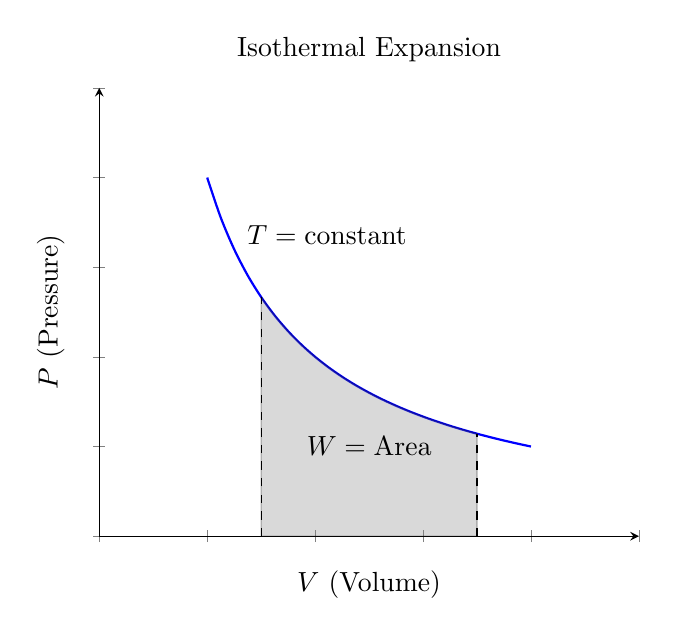
\begin{tikzpicture}
\begin{axis}[
    title={Isothermal Expansion},
    xlabel={$V$ (Volume)},
    ylabel={$P$ (Pressure)},
    xmin=0, xmax=5,
    ymin=0, ymax=5,
    xticklabels={}, yticklabels={},
    axis lines=left,
]
% Isothermal curve
\addplot[domain=1:4, smooth, thick, blue] {4/x} node[pos=0.2, above right, black] {$T = \text{constant}$};
% Area under the curve (Work)
\addplot[domain=1.5:3.5, fill=gray, opacity=0.3] {4/x} -- (axis cs:3.5,0) -- (axis cs:1.5,0) -- cycle;
% Labels
\draw [dashed] (axis cs:1.5,0) -- (axis cs:1.5, {4/1.5});
\draw [dashed] (axis cs:3.5,0) -- (axis cs:3.5, {4/3.5});
\node at (axis cs:1.5, -0.3) {$V_i$};
\node at (axis cs:3.5, -0.3) {$V_f$};
\node at (axis cs:2.5, 1) {$W = \text{Area}$};
\end{axis}
\end{tikzpicture}
\caption{A P-V diagram for an isothermal expansion.}
\end{figure}

\begin{itemize}
    \item \textbf{Energy Changes:}
    \begin{enumerate}
        \item \textbf{Internal Energy ($\Delta U$):} Since $\Delta U = nC_v\Delta T$ and $\Delta T = 0$, the internal energy change is $\mathbf{\Delta U = 0}$.
        \item \textbf{First Law:} $\Delta U = Q - W$ becomes $0 = Q - W$.
        \item \textbf{Conclusion: $Q = W$}
    \end{enumerate}
    \item \textbf{What it means:} Any heat ($Q$) added to the system is immediately converted into work ($W$) done by the system (expansion). All work done on the system (compression) is immediately released as heat.
    \item \textbf{Work Equation:}
    \begin{align*}
        W &= \int P \, dV = \int_{V_i}^{V_f} \frac{nRT}{V} \, dV \\
        W &= nRT \ln\left(\frac{V_f}{V_i}\right)
    \end{align*}
\end{itemize}

\subsection{Example: Isothermal Expansion}
\textbf{Question:} 2 moles of an ideal gas expand isothermally at $\SI{300}{K}$ from a volume of $\SI{10}{L}$ to $\SI{20}{L}$. Find $W$, $Q$, and $\Delta U$. ($R = \SI{8.314}{J/mol\cdot K}$)

\textbf{Solution:}
\begin{enumerate}
    \item \textbf{$\Delta U$:} It's \textbf{isothermal}, so $\Delta T = 0$. Therefore, $\mathbf{\Delta U = \SI{0}{J}}$.
    \item \textbf{$W$:} Use the work equation.
    \begin{align*}
        W &= nRT \ln(V_f / V_i) \\
        W &= (\SI{2}{mol}) \times (\SI{8.314}{J/mol\cdot K}) \times (\SI{300}{K}) \times \ln(\SI{20}{L} / \SI{10}{L}) \\
        W &= (4988.4) \times \ln(2) \\
        W &\approx (4988.4) \times (0.693) \\
        \mathbf{W} &\approx \mathbf{+\SI{3457}{J}} \text{ (Positive, because the gas expanded and did work).}
    \end{align*}
    \item \textbf{$Q$:} From the First Law for this process, $Q = W$.
    \begin{itemize}
        \item $\mathbf{Q = +\SI{3457}{J}}$ (Positive, because heat had to be added to keep the temperature from dropping).
    \end{itemize}
\end{enumerate}

\hrule

\section{Process 2: Adiabatic ("Insulated")}
\begin{itemize}
    \item \textbf{Definition:} A process with \textbf{no heat transfer}.
    \begin{itemize}
        \item $\mathbf{Q = 0}$
        \item Imagine the system is in a perfect thermos or the process happens so fast that heat has no time to flow.
    \end{itemize}
\end{itemize}

\begin{figure}[h]
\centering
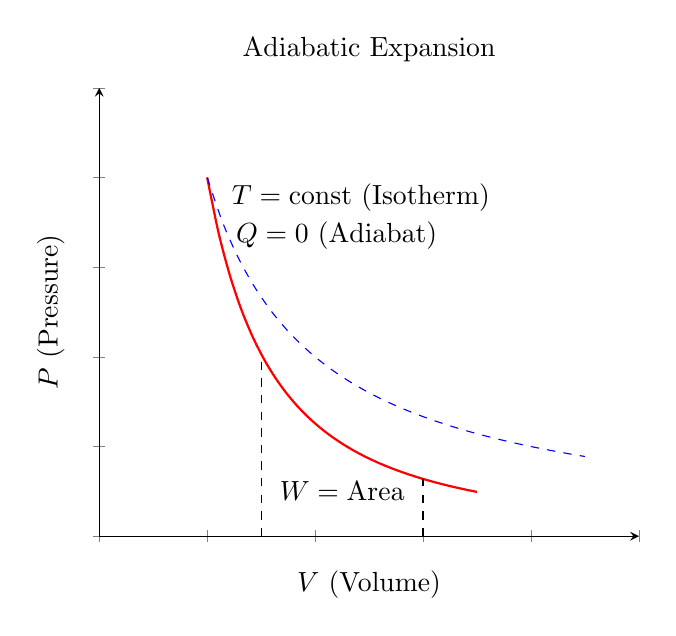
\begin{tikzpicture}
\begin{axis}[
    title={Adiabatic Expansion},
    xlabel={$V$ (Volume)},
    ylabel={$P$ (Pressure)},
    xmin=0, xmax=5,
    ymin=0, ymax=5,
    xticklabels={}, yticklabels={},
    axis lines=left,
]
% Adiabatic curve (steeper)
\addplot[domain=1:3.5, smooth, thick, red] {4/(x^1.67)} node[pos=0.2, above right, black] {$Q = 0 \text{ (Adiabat)}$};
% Isothermal curve (for comparison)
\addplot[domain=1:4.5, smooth, dashed, blue] {4/x} node[pos=0.1, above right, black] {$T = \text{const (Isotherm)}$};
% Labels
\draw [dashed] (axis cs:1.5,0) -- (axis cs:1.5, {4/(1.5^1.67)});
\draw [dashed] (axis cs:3.0,0) -- (axis cs:3.0, {4/(3.0^1.67)});
\node at (axis cs:1.5, -0.3) {$V_i$};
\node at (axis cs:3.0, -0.3) {$V_f$};
\node at (axis cs:2.25, 0.5) {$W = \text{Area}$};
\end{axis}
\end{tikzpicture}
\caption{A P-V diagram for an adiabatic expansion, showing it is steeper than an isotherm.}
\end{figure}

\begin{itemize}
    \item \textbf{Energy Changes:}
    \begin{enumerate}
        \item \textbf{Heat ($Q$):} By definition, $\mathbf{Q = 0}$.
        \item \textbf{First Law:} $\Delta U = Q - W$ becomes $\Delta U = 0 - W$.
        \item \textbf{Conclusion: $\Delta U = -W$}
    \end{enumerate}
    \item \textbf{What it means:}
    \begin{itemize}
        \item \textbf{Expansion ($W > 0$):} The gas does work ($W$). Since no heat $Q$ comes in, it must use its \textit{own} internal energy. $\Delta U$ is negative, so the \textbf{temperature drops}.
        \item \textbf{Compression ($W < 0$):} Work is done on the gas. This work energy is added directly to its internal energy. $\Delta U$ is positive, so the \textbf{temperature rises}.
    \end{itemize}
    \item \textbf{Adiabatic Index ($\gamma$):} This ratio is critical for adiabatic processes.
        $$ \gamma = \frac{C_p}{C_v} $$
    \begin{itemize}
        \item Monatomic: $\gamma = (5/2)R / (3/2)R = 5/3 \approx 1.67$
        \item Diatomic: $\gamma = (7/2)R / (5/2)R = 7/5 = 1.40$
    \end{itemize}
    \item \textbf{Process Equations:} (Use these to find $P, V, T$ at the end of the process)
        $$ P_iV_i^\gamma = P_fV_f^\gamma $$
        $$ T_iV_i^{\gamma-1} = T_fV_f^{\gamma-1} $$
    \item \textbf{Work Equation:}
        $$ W = \frac{P_iV_i - P_fV_f}{\gamma - 1} \quad \text{or} \quad W = -nC_v(T_f - T_i) $$
\end{itemize}

\subsection{Example: Adiabatic Compression}
\textbf{Question:} A cylinder of air (a diatomic gas, $\gamma = 1.4$) is compressed adiabatically from $P_i = \SI{1}{atm}$, $T_i = \SI{300}{K}$ to $\frac{1}{10}$th of its original volume ($V_f = V_i / 10$). Find the final temperature ($T_f$), $W$, and $\Delta U$ for 1 mole of gas.

\textbf{Solution:}
\begin{enumerate}
    \item \textbf{Find $T_f$:} Use the $T-V$ relationship.
    \begin{align*}
        T_iV_i^{\gamma-1} &= T_fV_f^{\gamma-1} \implies T_f = T_i \left(\frac{V_i}{V_f}\right)^{\gamma-1} \\
        \gamma - 1 &= 1.4 - 1 = 0.4 \\
        T_f &= (\SI{300}{K}) \times \left(\frac{V_i}{V_i/10}\right)^{0.4} = (\SI{300}{K}) \times (10)^{0.4} \\
        T_f &\approx 300 \times 2.51 \approx \mathbf{\SI{754}{K}} \text{ (Temperature rose significantly!)}
    \end{align*}
    \item \textbf{Find $\Delta U$:} Now that we have $\Delta T$, this is easiest. (For air, $C_v = \frac{5}{2}R$)
    \begin{align*}
        \Delta U &= nC_v\Delta T = (\SI{1}{mol}) \times (\frac{5}{2} \times \SI{8.314}{J/mol\cdot K}) \times (\SI{754}{K} - \SI{300}{K}) \\
        \Delta U &= (1) \times (20.785) \times (454) \approx \mathbf{+\SI{9435}{J}}
    \end{align*}
    \item \textbf{Find $W$:} From the First Law for this process, $W = -\Delta U$.
    \begin{itemize}
        \item $\mathbf{W = -\SI{9435}{J}}$ (Negative, as work was done \textit{on} the gas to compress it).
    \end{itemize}
\end{enumerate}

\hrule

\section{Entropy ($\Delta S$)}
\begin{itemize}
    \item \textbf{Concept:} A measure of \textbf{disorder}, \textbf{randomness}, or the spreading of energy.
    \item \textbf{The Second Law of Thermodynamics:} The total entropy of the universe (system + surroundings) \textbf{always increases} for any real (spontaneous) process. $\Delta S_{\text{universe}} > 0$.
    \item \textbf{Calculating Entropy Change:} The change in entropy is defined for a \textit{reversible} process at a constant temperature $T$.
        $$ \Delta S = \frac{Q_{\text{rev}}}{T} $$
    \begin{itemize}
        \item $Q_{\text{rev}}$ = Heat added in a reversible (slow, ideal) process.
        \item $T$ = Absolute temperature (in Kelvin).
        \item Units: Joules per Kelvin (\SI{}{J/K}).
    \end{itemize}
    \item \textbf{What it means:}
    \begin{itemize}
        \item If you add heat ($Q > 0$), you increase the disorder ($\Delta S > 0$).
        \item Adding the \textit{same} amount of heat to a \textit{cold} system (low $T$) causes \textit{more} of an entropy change than adding it to a \textit{hot} system (high $T$).
    \end{itemize}
\end{itemize}

\subsection{Example 1: Entropy of Melting}
\textbf{Question:} Calculate the change in entropy when $\SI{50}{g}$ of ice melts at $\SI{0}{^\circ C}$ ($\SI{273.15}{K}$). The latent heat of fusion for water is $\SI{334}{J/g}$.

\textbf{Solution:}
\begin{enumerate}
    \item \textbf{Find $Q$:} Melting is a constant-temperature process.
    \begin{itemize}
        \item $Q = \text{mass} \times L_f = (\SI{50}{g}) \times (\SI{334}{J/g}) = \SI{16700}{J}$
    \end{itemize}
    \item \textbf{Find $\Delta S$:} Use the entropy equation.
    \begin{align*}
        \Delta S &= Q / T \\
        \Delta S &= \SI{16700}{J} / \SI{273.15}{K} \approx \mathbf{+\SI{61.1}{J/K}}
    \end{align*}
    (Entropy increased, which makes sense: liquid water is more disordered than solid ice).
\end{enumerate}

\subsection{Example 2: Entropy of Isothermal Expansion}
\textbf{Question:} What was the entropy change \textit{of the gas} in our first example (the isothermal expansion)?

\textbf{Solution:}
\begin{enumerate}
    \item \textbf{Recall from Example 1:} The process was at a constant $T = \SI{300}{K}$ and we added $Q = +\SI{3457}{J}$ of heat.
    \item \textbf{Find $\Delta S$:}
    \begin{align*}
        \Delta S &= Q / T \\
        \Delta S &= \SI{3457}{J} / \SI{300}{K} \approx \mathbf{+\SI{11.5}{J/K}}
    \end{align*}
    (Entropy increased, which makes sense: the gas spread out into a larger volume, increasing its disorder).
\end{enumerate}

\hrule

\section{Summary Table}

\begin{center}
\begin{tabular}{l | l | l | l | l | l}
\toprule
\textbf{Process} & \textbf{Condition} & \textbf{Internal Energy ($\Delta U$)} & \textbf{Heat ($Q$)} & \textbf{Work ($W$)} & \textbf{Entropy ($\Delta S_{\text{gas}}$)} \\
\midrule
\textbf{Isothermal} & $\Delta T = 0$ & $\mathbf{\Delta U = 0}$ & $Q = W$ & $W = nRT \ln(V_f/V_i)$ & $\Delta S = Q/T$ \\
\textbf{Adiabatic} & $Q = 0$ & $\Delta U = -W$ & $\mathbf{Q = 0}$ & $W = -nC_v\Delta T$ & $\mathbf{\Delta S = 0}$ (ideal) \\
\bottomrule
\end{tabular}
\end{center}

\hrule

\section{Integrative Problems: The Cyclic Process}
Cyclic processes are the foundation of engines and refrigerators. They are excellent for testing your understanding because the system returns to its starting point.

\textbf{Key Rules for a Full Cycle:}
\begin{itemize}
    \item The system's state ($P, V, T$) is the same at the end as the beginning.
    \item Since internal energy $\Delta U$ only depends on temperature, the total change for a full cycle is $\mathbf{\Delta U_{\text{cycle}} = 0}$.
    \item From the First Law ($\Delta U = Q - W$), this means $\mathbf{Q_{\text{net}} = W_{\text{net}}}$. The net heat absorbed equals the net work done.
    \item Since entropy $S$ is a state function, the total change for a full cycle is $\mathbf{\Delta S_{\text{cycle}} = 0}$.
\end{itemize}

\subsection{Problem 1: The "Iso-Adia-Iso" Cycle}
You have \textbf{1.0 mole of a monatomic ideal gas} that undergoes the following 3-step cycle.

\begin{figure}[h]
\centering
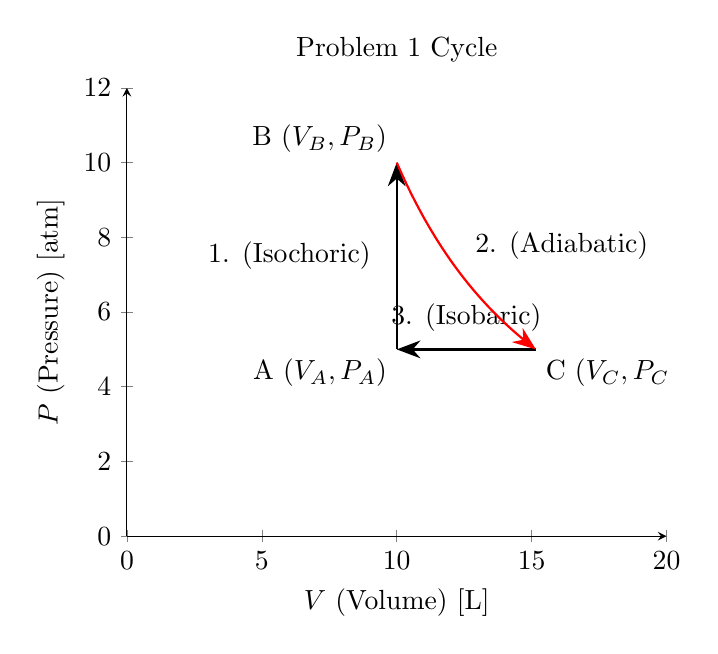
\begin{tikzpicture}
\begin{axis}[
    title={Problem 1 Cycle},
    xlabel={$V$ (Volume) [L]},
    ylabel={$P$ (Pressure) [atm]},
    xmin=0, xmax=20,
    ymin=0, ymax=12,
    axis lines=left,
    legend pos=outer north east
]
% Points
\coordinate (A) at (axis cs:10, 5);
\coordinate (B) at (axis cs:10, 10);
\coordinate (C) at (axis cs:15.16, 5);

% Nodes
\node[below left] at (A) {A ($V_A, P_A$)};
\node[above left] at (B) {B ($V_B, P_B$)};
\node[below right] at (C) {C ($V_C, P_C$)};

% A -> B (Isochoric)
\draw [thick, -{Stealth[length=3mm]}] (A) -- (B) node[midway, left, xshift=-2mm] {1. (Isochoric)};

% C -> A (Isobaric)
\draw [thick, -{Stealth[length=3mm]}] (C) -- (A) node[midway, above, yshift=1mm] {3. (Isobaric)};

% B -> C (Adiabatic)
\addplot[domain=10:15.16, smooth, thick, red, -{Stealth[length=3mm]}] {10*(10^1.667)/(x^1.667)} node[midway, above right, xshift=1mm, black] {2. (Adiabatic)};

\end{axis}
\end{tikzpicture}
\caption{P-V Diagram for the Integrative Problem 1.}
\end{figure}

\begin{itemize}
    \item \textbf{Gas Properties:} Monatomic $\implies C_v = \frac{3}{2}R$, $C_p = \frac{5}{2}R$, $\gamma = \frac{5}{3}$
    \item \textbf{Constants:} $R = \SI{8.314}{J/mol\cdot K}$ ($\SI{1}{L\cdot atm} = \SI{101.3}{J}$)
\end{itemize}

The cycle starts at \textbf{State A}:
\begin{itemize}
    \item $P_A = \SI{5.00}{atm}$
    \item $V_A = \SI{10.0}{L}$
\end{itemize}

\textbf{The Process:}
\begin{enumerate}
    \item \textbf{A $\to$ B:} The gas is heated at \textbf{constant volume (isochoric)} until its pressure doubles to $P_B = \SI{10.0}{atm}$.
    \item \textbf{B $\to$ C:} The gas expands \textbf{adiabatically ($Q=0$)} until it returns to its original pressure $P_C = \SI{5.00}{atm}$.
    \item \textbf{C $\to$ A:} The gas is compressed at \textbf{constant pressure (isobaric)} back to State A.
\end{enumerate}

\textbf{Your Tasks:}
\begin{enumerate}
    \item \textbf{Find $P, V, T$ for all 3 States.} (Hint: Find $T_A$ first using $PV=nRT$).
    \item \textbf{Calculate $W, Q, \Delta U,$ and $\Delta S$ for \textit{each step} (A$\to$B, B$\to$C, C$\to$A).}
    \item \textbf{Calculate $W_{\text{net}}, Q_{\text{net}}, \Delta U_{\text{cycle}},$ and $\Delta S_{\text{cycle}}$ for the \textit{entire cycle}.}
\end{enumerate}

\hrule

\subsection{Solution for Problem 1}

\subsubsection{1. $P, V, T$ for States A, B, C}
(Using $R = \SI{0.0821}{L\cdot atm/mol\cdot K}$ for $P,V,T$ calcs)

\begin{itemize}
    \item \textbf{State A:} $P_A = \SI{5.00}{atm}$, $V_A = \SI{10.0}{L}$.
        \begin{itemize}
            \item $T_A = \frac{P_A V_A}{nR} = \frac{(\SI{5.00}{atm} \times \SI{10.0}{L})}{(\SI{1}{mol} \times \SI{0.0821}{L\cdot atm/mol\cdot K})} = \mathbf{\SI{609}{K}}$
        \end{itemize}
    
    \item \textbf{State B:} $V_B = V_A = \SI{10.0}{L}$ (isochoric). $P_B = \SI{10.0}{atm}$.
        \begin{itemize}
            \item $T_B = \frac{P_B V_B}{nR} = \frac{(\SI{10.0}{atm} \times \SI{10.0}{L})}{(\SI{1}{mol} \times \SI{0.0821}{L\cdot atm/mol\cdot K})} = \mathbf{\SI{1218}{K}}$
        \end{itemize}
        
    \item \textbf{State C:} $P_C = \SI{5.00}{atm}$ (isobaric). From B$\to$C (adiabatic, $\gamma=5/3$).
    \begin{itemize}
        \item Use $P_B V_B^\gamma = P_C V_C^\gamma \implies V_C = V_B \left(\frac{P_B}{P_C}\right)^{1/\gamma}$
        \item $V_C = (\SI{10.0}{L}) \times \left(\frac{\SI{10.0}{atm}}{\SI{5.00}{atm}}\right)^{1 / (5/3)} = (\SI{10.0}{L}) \times (2)^{3/5}$
        \item $V_C \approx (\SI{10.0}{L}) \times (1.516) = \mathbf{\SI{15.16}{L}}$
        \item $T_C = \frac{P_C V_C}{nR} = \frac{(\SI{5.00}{atm} \times \SI{15.16}{L})}{(\SI{1}{mol} \times \SI{0.0821}{L\cdot atm/mol\cdot K})} = \mathbf{\SI{923}{K}}$
    \end{itemize}
\end{itemize}
\textbf{Summary of States:}
\begin{itemize}
    \item A: ($\SI{5.00}{atm}$, $\SI{10.0}{L}$, $\SI{609}{K}$)
    \item B: ($\SI{10.0}{atm}$, $\SI{10.0}{L}$, $\SI{1218}{K}$)
    \item C: ($\SI{5.00}{atm}$, $\SI{15.16}{L}$, $\SI{923}{K}$)
\end{itemize}

\subsubsection{2. $W, Q, \Delta U, \Delta S$ for Each Step}
($C_v = \frac{3}{2}R = \SI{12.47}{J/mol\cdot K}$; $C_p = \frac{5}{2}R = \SI{20.79}{J/mol\cdot K}$)

\paragraph{Step A $\to$ B (Constant Volume):}
\begin{itemize}
    \item $\Delta V = 0 \implies \mathbf{W = \SI{0}{J}}$
    \item $\Delta T = T_B - T_A = 1218 - 609 = \SI{609}{K}$
    \item $\Delta U = nC_v\Delta T = (1)(\SI{12.47}{J/mol\cdot K})(\SI{609}{K}) = \mathbf{+\SI{7595}{J}}$
    \item $Q = \Delta U + W = \SI{7595}{J} + 0 = \mathbf{+\SI{7595}{J}}$
    \item $\Delta S = nC_v \ln(T_B / T_A) = (1)(12.47) \ln(1218 / 609) = (12.47) \ln(2) = \mathbf{+\SI{8.64}{J/K}}$
\end{itemize}

\paragraph{Step B $\to$ C (Adiabatic):}
\begin{itemize}
    \item $\mathbf{Q = \SI{0}{J}}$ (by definition)
    \item $\Delta T = T_C - T_B = 923 - 1218 = \SI{-295}{K}$
    \item $\Delta U = nC_v\Delta T = (1)(12.47)(-295) = \mathbf{-\SI{3679}{J}}$
    \item $W = -\Delta U = \mathbf{+\SI{3679}{J}}$ (Gas expanded, did work)
    \item $\mathbf{\Delta S = \SI{0}{J/K}}$ (Reversible adiabatic process)
\end{itemize}

\paragraph{Step C $\to$ A (Constant Pressure):}
\begin{itemize}
    \item $\Delta T = T_A - T_C = 609 - 923 = \SI{-314}{K}$
    \item $W = P\Delta V = P_A (V_A - V_C) = (\SI{5.00}{atm}) \times (\SI{10.0}{L} - \SI{15.16}{L})$
    \item $W = (\SI{5.00}{atm}) \times (\SI{-5.16}{L}) = \SI{-25.8}{L\cdot atm}$
    \item $W = (\SI{-25.8}{L\cdot atm}) \times (\SI{101.3}{J/L\cdot atm}) = \mathbf{-\SI{2614}{J}}$ (Gas compressed)
    \item $\Delta U = nC_v\Delta T = (1)(12.47)(-314) = \mathbf{-\SI{3916}{J}}$
    \item $Q = \Delta U + W = -3916 + (-2614) = \mathbf{-\SI{6530}{J}}$ (Heat released)
    \item $\Delta S = nC_p \ln(T_A / T_C) = (1)(20.79) \ln(609 / 923) = (20.79)(-0.417) = \mathbf{-\SI{8.67}{J/K}}$
\end{itemize}

\subsubsection{3. Totals for the Entire Cycle}
\begin{itemize}
    \item $\mathbf{\Delta U_{\text{cycle}}}$ = $\Delta U_{AB} + \Delta U_{BC} + \Delta U_{CA} = (+7595) + (-3679) + (-3916) = \mathbf{0} \text{ (approx)}$
    \item $\mathbf{W_{\text{net}}}$ = $W_{AB} + W_{BC} + W_{CA} = 0 + (+3679) + (-2614) = \mathbf{+\SI{1065}{J}}$
    \item $\mathbf{Q_{\text{net}}}$ = $Q_{AB} + Q_{BC} + Q_{CA} = (+7595) + 0 + (-6530) = \mathbf{+\SI{1065}{J}}$
    \item \textbf{Check:} $Q_{\text{net}} = W_{\text{net}}$. The First Law is satisfied.
    \item $\mathbf{\Delta S_{\text{cycle}}}$ = $\Delta S_{AB} + \Delta S_{BC} + \Delta S_{CA} = (+8.64) + 0 + (-8.67) = \mathbf{-0.03} \text{ (approx. 0)}$
    \item (As expected, since U and S are state functions, their net change in a cycle is zero).
\end{itemize}

\hrule

\section{Problem 2: The Ideal Carnot Engine}
This problem follows the path of an ideal engine, which is the perfect way to combine all the concepts.

You have \textbf{1.0 mole of a diatomic ideal gas} (like N$_2$). The gas starts at \textbf{State A} and undergoes the following 4-step reversible cycle:
\begin{itemize}
    \item \textbf{Gas Properties:} Diatomic $\implies C_v = \frac{5}{2}R$, $C_p = \frac{7}{2}R$, $\gamma = \frac{7}{5} = 1.4$
    \item \textbf{Constants:} $R = \SI{8.314}{J/mol\cdot K}$
\end{itemize}

% --- CORRECTED CARNOT CYCLE FIGURE ---
\centering
\begin{tikzpicture}[scale=1.0]

% Axes
\draw[->] (0,0) -- (7,0) node[right] {$V$};
\draw[->] (0,0) -- (0,5) node[above] {$P$};

% Carnot cycle with strongly curved segments
\draw[thick]
  (1.0, 4.0) node[above left] {A}
  .. controls (1.5, 3.0) and (2.5, 2.6) ..
  (3.2, 2.4) node[above right] {B}   % A->B: clearly curved isothermal
  .. controls (3.3, 1.6) and (3.5, 1.0) ..
  (3.6, 0.7) node[below right] {C}   % B->C: sharply curved adiabatic
  .. controls (2.7, 1.1) and (1.8, 1.8) ..
  (1.4, 2.3) node[below left] {D}    % C->D: curved isothermal
  .. controls (1.1, 3.2) and (1.0, 3.7) ..
  cycle;                             % D->A: sharply curved adiabatic

\end{tikzpicture}
% --- END OF CORRECTED FIGURE ---


\textbf{The Process:}
The cycle operates between two heat reservoirs at $T_H = \SI{600}{K}$ and $T_C = \SI{300}{K}$.

\begin{enumerate}
    \item \textbf{A $\to$ B:} The gas starts at $T_A = \SI{600}{K}$ and $V_A = \SI{5.0}{L}$. It expands \textbf{isothermally} at $T_H = \SI{600}{K}$ to a new volume $V_B = \SI{10.0}{L}$. It absorbs heat $Q_H$ from the hot reservoir.
    \item \textbf{B $\to$ C:} The gas expands \textbf{adiabatically ($Q=0$)}, cooling down from $T_H$ to $T_C = \SI{300}{K}$.
    \item \textbf{C $\to$ D:} The gas is compressed \textbf{isothermally} at $T_C = \SI{300}{K}$. It expels heat $Q_C$ to the cold reservoir.
    \item \textbf{D $\to$ A:} The gas is compressed \textbf{adiabatically ($Q=0$)}, heating back up from $T_C$ to $T_H = \SI{600}{K}$ and returning to State A.
\end{enumerate}

\textbf{Your Tasks:}

\begin{enumerate}
    \item Find the volumes at State C ($V_C$) and State D ($V_D$).
    \item Calculate $\Delta U$, $Q$, $W$, and $\Delta S$ for all four steps.
    \item Find the net work ($W_{\text{net}}$) done by the engine in one cycle.
    \item Calculate the thermal efficiency ($\eta$) of the engine.
\end{enumerate}

\hrule

\subsection{Solution for Problem 2}

First, let's list our gas properties:
\begin{itemize}
    \item $n = 1.0 \text{ mol}$
    \item $R = \SI{8.314}{J/mol\cdot K}$
    \item $C_v = \frac{5}{2}R = \frac{5}{2}(\SI{8.314}{J/mol\cdot K}) = \SI{20.785}{J/mol\cdot K}$
    \item $\gamma = 1.4 \implies \gamma - 1 = 0.4$
\end{itemize}

\textbf{Summary of States:}
\begin{itemize}
    \item \textbf{A:} $T_A = \SI{600}{K}$, $V_A = \SI{5.0}{L}$
    \item \textbf{B:} $T_B = \SI{600}{K}$, $V_B = \SI{10.0}{L}$
    \item \textbf{C:} $T_C = \SI{300}{K}$, $V_C = ?$
    \item \textbf{D:} $T_D = \SI{300}{K}$, $V_D = ?$
\end{itemize}


\subsubsection{1. Find $V_C$ and $V_D$}
\begin{itemize}
    \item \textbf{For B $\to$ C (Adiabatic):} We use the $T-V$ relationship: $T_B V_B^{\gamma-1} = T_C V_C^{\gamma-1}$
    \begin{align*}
        (\SI{600}{K}) \times (\SI{10.0}{L})^{1.4-1} &= (\SI{300}{K}) \times (V_C)^{1.4-1} \\
        600 \times (10.0)^{0.4} &= 300 \times (V_C)^{0.4} \\
        2 \times (10.0)^{0.4} &= (V_C)^{0.4} \quad \text{(Divide by 300)} \\
        V_C &= (10.0) \times (2)^{1/0.4} = (10.0) \times (2)^{2.5} \\
        V_C &\approx (10.0) \times (5.657) \\
        \mathbf{V_C} &\approx \mathbf{\SI{56.57}{L}}
    \end{align*}

    \item \textbf{For D $\to$ A (Adiabatic):} We use the same relationship: $T_D V_D^{\gamma-1} = T_A V_A^{\gamma-1}$
    \begin{align*}
        (\SI{300}{K}) \times (V_D)^{0.4} &= (\SI{600}{K}) \times (\SI{5.0}{L})^{0.4} \\
        (V_D)^{0.4} &= 2 \times (\SI{5.0}{L})^{0.4} \quad \text{(Divide by 300)} \\
        V_D &= (5.0) \times (2)^{2.5} \\
        V_D &\approx (5.0) \times (5.657) \\
        \mathbf{V_D} &\approx \mathbf{\SI{28.28}{L}}
    \end{align*}
\end{itemize}

\subsubsection{2. Calculate $\Delta U, Q, W,$ and $\Delta S$ for Each Step}
\paragraph{Step A $\to$ B (Isothermal Expansion at $\SI{600}{K}$):}
\begin{itemize}
    \item $\Delta T = 0 \implies \mathbf{\Delta U = 0 \text{ J}}$
    \item $W = nRT_H \ln(V_B / V_A) = (1.0)(\SI{8.314}{J/mol\cdot K})(\SI{600}{K}) \times \ln(\SI{10.0}{L} / \SI{5.0}{L})$
    \item $W = (4988.4) \times \ln(2) \approx \mathbf{+\SI{3457}{J}}$
    \item $Q = W \implies \mathbf{Q_H = +\SI{3457}{J}}$ (This is the heat \textit{absorbed} from the hot reservoir)
    \item $\Delta S = Q_H / T_H = \SI{3457}{J} / \SI{600}{K} = \mathbf{+\SI{5.76}{J/K}}$
\end{itemize}

\paragraph{Step B $\to$ C (Adiabatic Expansion):}
\begin{itemize}
    \item $\mathbf{Q = 0 \text{ J}}$ (by definition)
    \item $\Delta T = T_C - T_B = \SI{300}{K} - \SI{600}{K} = \SI{-300}{K}$
    \item $\Delta U = nC_v\Delta T = (1.0 \text{ mol})(\SI{20.785}{J/mol\cdot K})(\SI{-300}{K}) = \mathbf{-\SI{6236}{J}}$
    \item $W = -\Delta U \implies \mathbf{W = +\SI{6236}{J}}$ (The gas does work using its own energy)
    \item $\mathbf{\Delta S = 0 \text{ J/K}}$ (for any reversible, adiabatic process)
\end{itemize}

\paragraph{Step C $\to$ D (Isothermal Compression at $\SI{300}{K}$):}
\begin{itemize}
    \item $\Delta T = 0 \implies \mathbf{\Delta U = 0 \text{ J}}$
    \item $W = nRT_C \ln(V_D / V_C) = (1.0)(\SI{8.314}{J/mol\cdot K})(\SI{300}{K}) \times \ln(\SI{28.28}{L} / \SI{56.57}{L})$
    \item $W = (2494.2) \times \ln(0.5) = (2494.2) \times (-0.693) \approx \mathbf{-\SI{1728}{J}}$
    \item $Q = W \implies \mathbf{Q_C = -\SI{1728}{J}}$ (This is the heat \textit{expelled} to the cold reservoir)
    \item $\Delta S = Q_C / T_C = \SI{-1728}{J} / \SI{300}{K} = \mathbf{-\SI{5.76}{J/K}}$
\end{itemize}

\paragraph{Step D $\to$ A (Adiabatic Compression):}
\begin{itemize}
    \item $\mathbf{Q = 0 \text{ J}}$ (by definition)
    \item $\Delta T = T_A - T_D = \SI{600}{K} - \SI{300}{K} = \SI{+300}{K}$
    \item $\Delta U = nC_v\Delta T = (1.0 \text{ mol})(\SI{20.785}{J/mol\cdot K})(\SI{+300}{K}) = \mathbf{+\SI{6236}{J}}$
    \item $W = -\Delta U \implies \mathbf{W = -\SI{6236}{J}}$ (Work is done \textit{on} the gas to heat it)
    \item $\mathbf{\Delta S = 0 \text{ J/K}}$ (for any reversible, adiabatic process)
\end{itemize}

\subsubsection{3. Find the Net Work ($W_{\text{net}}$)}
$W_{\text{net}}$ is the sum of the work from all four steps.
\begin{itemize}
    \item $W_{\text{net}} = W_{AB} + W_{BC} + W_{CD} + W_{DA}$
    \item $W_{\text{net}} = (+\SI{3457}{J}) + (+\SI{6236}{J}) + (-\SI{1728}{J}) + (-\SI{6236}{J})$
    \item $W_{\text{net}} = \SI{3457}{J} - \SI{1728}{J} = \mathbf{+\SI{1729}{J}}$
\end{itemize}
\textbf{Check with First Law:}
\begin{itemize}
    \item $Q_{\text{net}} = Q_H + Q_C = (+\SI{3457}{J}) + (-\SI{1728}{J}) = \mathbf{+\SI{1729}{J}}$
    \item $\Delta U_{\text{cycle}} = \Delta U_{AB} + \Delta U_{BC} + \Delta U_{CD} + \Delta U_{DA} = 0 + (-\SI{6236}{J}) + 0 + (+\SI{6236}{J}) = \mathbf{0 \text{ J}}$
    \item Since $\Delta U_{\text{cycle}} = Q_{\text{net}} - W_{\text{net}}$, we get $0 = (\SI{1729}{J}) - (\SI{1729}{J})$, which is correct.
\end{itemize}

\subsubsection{4. Calculate the Thermal Efficiency ($\eta$)}
Efficiency is what you get (Net Work) divided by what you paid for (Heat from the hot reservoir, $Q_H$).
\begin{itemize}
    \item $\eta = \frac{W_{\text{net}}}{Q_H} = \frac{\SI{1729}{J}}{\SI{3457}{J}} \approx 0.50$
    \item $\mathbf{\eta = 50\%}$
\end{itemize}
\textbf{Final Check (Carnot's Formula):}
The maximum theoretical efficiency (the Carnot efficiency) is given \textit{only} by the temperatures.
\begin{itemize}
    \item $\eta_{\text{Carnot}} = 1 - \frac{T_C}{T_H}$
    \item $\eta_{\text{Carnot}} = 1 - \frac{\SI{300}{K}}{\SI{600}{K}} = 1 - 0.5 = 0.50$
    \item $\mathbf{\eta = 50\%}$
\end{itemize}
Our calculations match the theoretical formula perfectly.


\end{document}